% HEADER
\documentclass[class=article, crop=false]{standalone}
\usepackage{00_Preamble/frr_preamble}

% Packages
\usepackage{titlesec}
\usepackage{hyperref}
\usepackage{float}
\usepackage{graphics}
\usepackage{placeins}
\usepackage{adjustbox}
% END HEADER

\begin{document}
	\subsection{Technical Management}
	\label{subsec:technical_management}
	
	\subsubsection{Energy and Mass Budget}
	In order to ensure that all of the subsystems were considered and shared resources equally, power and mass were budgeted between the systems prior to conceptualization. The energy and mass budgets are presented in Tables \ref{table:mass_budget} and \ref{table:energy_budget}, respectively.
	
\FloatBarrier
	\begin{table}[h]
	\scriptsize
	\parbox{.45\linewidth}{
	\centering
	\begin{tabular}{ | r | c | }
 	\hline		
 	\rowcolor[gray]{0.8}
 		\textbf{Subsystem} & \textbf{Estimated Weight (kg)} \\
 		\hline\hline
 		\textbf{Excavation} & 30 \\
 		\hline
 		\textbf{Depositing} & 26 \\
 		\hline
 		\textbf{Frame} & 12 \\
 		\hline
 		\textbf{Total} & 68 \\
 		\hline
	\end{tabular}
	\caption{Mass Budget Summary}
		\label{table:mass_budget}
	}
	\hfill
	\parbox{.45\linewidth}{
	\centering
	\begin{tabular}{ | r | c | }
 	\hline		
 	\rowcolor[gray]{0.8}
 		\textbf{Subsystem} & \textbf{Estimated Energy Usage (Ah)} \\
 		\hline\hline
 		\textbf{Excavation} & 6.6 \\
 		\hline
 		\textbf{Depositing} & 2 \\
 		\hline
 		\textbf{Frame} & 18.7 \\
 		\hline
 		\textbf{Other} & 18.7 \\
 		\hline
 		\textbf{Total} & 29.7 \\
 		\hline
	\end{tabular}
	\caption{Energy Budget Summary}
		\label{table:energy_budget}
	}
	\end{table}
	\FloatBarrier
	
	\subsubsection{Interface Management}
	When designing each subsystem on the robot, interfaces between the subsystems were clearly defined in order to ensure that the system integration process occurs without errors. Well-defined interfaces also improve the ability to swap in new parts in the case of failures.
	
	\vspace*{0.1in}
	\noindent\textbf{\underline{Frame Interfaces}}
	
	The frame was designed to be modular and easy to assemble. Due to tolerances in custom fabricated parts, it was important to leave room for error in the assembly process. The base frame consists of aluminum extrusions connected together by mounting plates and T-nuts. The T-nuts allow the connection points to be adjusted continuously along the aluminum extrusions as needed. The motor mounts that attach the wheels to the frame are also connected with T-nuts. This allows the wheel’s position to be modified along the length of the frame so that the wheel spacing can be optimized for the best turning radius during the testing phase. The vertical conveyor supports on the frame are connected by brackets so that the conveyor angle and length can be adjusted to reach the team-defined requirement of depositing gravel 3 inches above the collection bin. The linear actuators are attached to the frame by adjustable brackets that allow the final auger digging angle to be modified. 
	
	\vspace*{0.1in}
	\newpage
	\noindent\textbf{\underline{Electronics Interfaces}}
	
	In order to have good interfaces for the electronic signals, a custom PCB was designed to route electrical signals (See Figure \ref{fig:pcb}). The PCB would help to reduce noise from electromagnetic radiation as well as wiring messes. All batteries, busbar, controllers, computers, and relays are housed inside a box near the back of the robot. The breakers and the emergency button are attached to the top of the box. The box is bolted to the frame. The electrical connections to the motors are detachable with XT-90 connectors, which allows the electrical box to be removed easily. All sensors and SoCs are powered directly or indirectly with a 5V- or 12V-boost converter, which are powered directly from all four batteries.

	\FloatBarrier
	\begin{wrapfigure}{r}{0.6\textwidth}
		\centering
		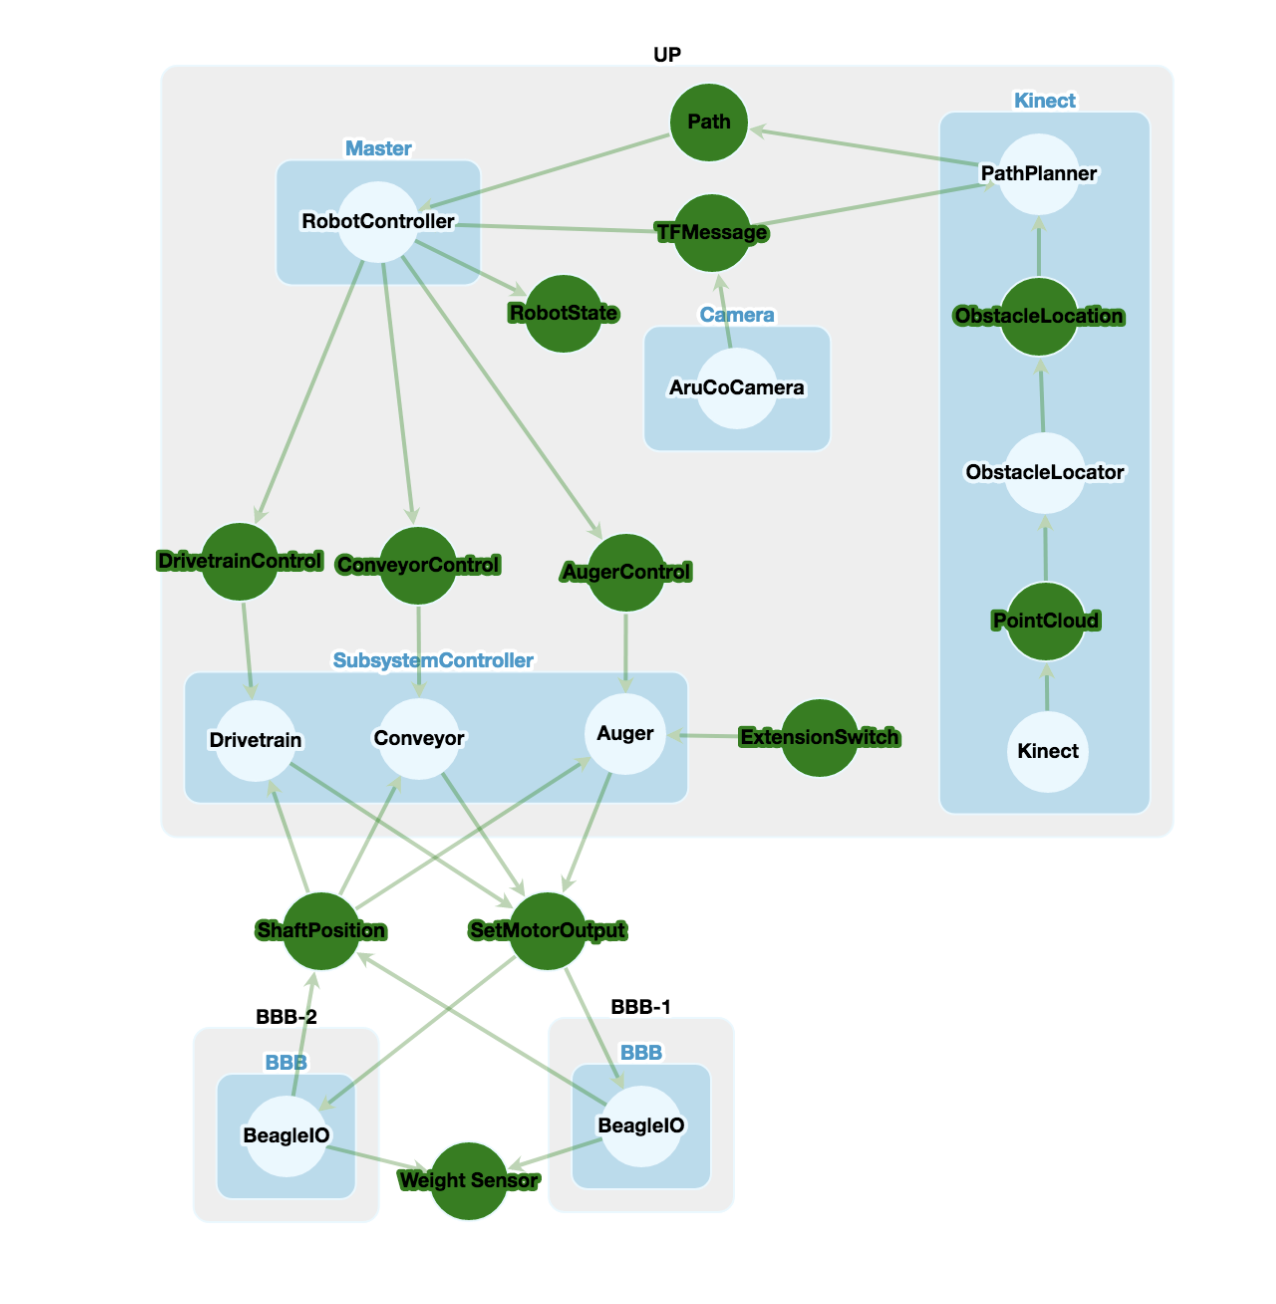
\includegraphics[width=1\linewidth]{09_Figures/programming_interfaces.png}
		\caption{ROSMOD Software Interface Diagram}
		\label{fig:system_hierarchy}
	\end{wrapfigure}
	\FloatBarrier
	
	All motors are driven indirectly from a PWM signal that is generated from a BeagleBone Blue. The PWM signal for the auger and conveyor is read by an AmpFlow motor controller. The PWM signals for the drive motors are read by the VEX VictorSPX motor controllers. The signal for the lead screw is read by a ceiling fan speed controller. Each motor (except for the lead screw motor) is equipped with an encoder that can determine its relative rotation and its angular velocity. The drive encoders collect odometry measurements for the autonomy algorithms, and the auger and conveyor encoders provide data for autonomy state machine. 
	
	The sensor data from the Kinect are processed with an obstacle detection algorithm, and the webcam data are processed with OpenCV fiducial recognition. Both algorithms are performed on the UP board. These data help determine the robot’s pose and the obstacles’ locations for the autonomy algorithm. 
	
	\vspace*{0.1in}
	\noindent\textbf{\underline{Software Interfaces}}
	
	A diagram for the software interfaces generated in ROSMOD is shown in Figure \ref{fig:system_hierarchy}. Each green circle in the diagram represents a message that serves as the interface between the various nodes (the white circles). Messages define how different components of the controller communicate with each other. The robot controller connects the autonomy controller and tele-operator controller to the sensors and motor controllers across the robot. Data from each sensor is published on a unique message and subscribed to by other components. 
	
	Components subscribe to individual messages, making them agnostic to the component sending the messages. Therefore, each sub-system can abstract control of its individual motors and sensors to provide one interface for controlling. This abstraction allows control schemes where subsystems like the drive have only a generalized interface for accepting speed commands, which can be sent by either the autonomy controller or operator input. In addition to providing the ability for multiple control inputs, the generalized interface also allows for easy debugging and data collection as you can easily use ROS tools to observe all messages being sent to verify functionality.
		
	\FloatBarrier
	\begin{figure}[h]
		\centering
		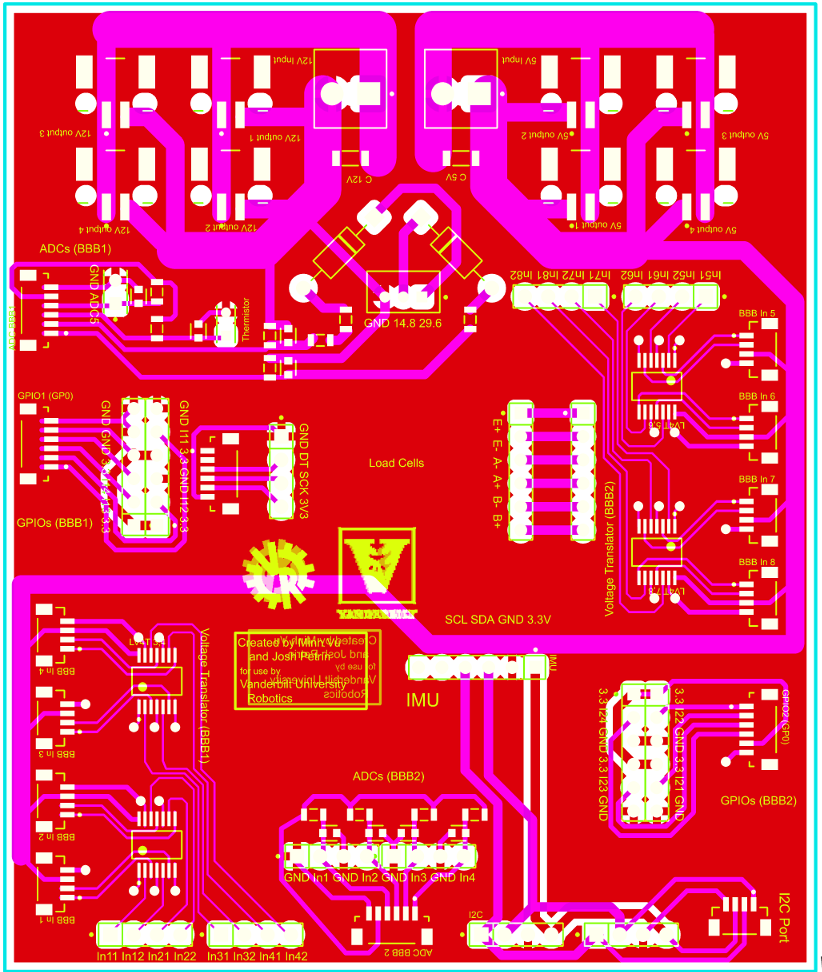
\includegraphics[width=0.6\linewidth]{09_Figures/pcb.jpg}
		\caption{The Printed Circuit Board, which contains many of the robot's data signals.}
		\label{fig:pcb}
	\end{figure}
	\FloatBarrier
	
	
\end{document}
